\graphicspath{{./content/seg_assessment/figures/}}
\section{Segmentation assessment}\label{section:assessment}
Comparing all the methodologies reviewed in section~\ref{section:userInteraction} is rather cumbersome. The lack of a common framework for assessing the methodologies remains unaddressed, especially due to the absence of a public image dataset despite its being highly demanded by the scientific community~\cite{Noble:2006p1734,Noble:2009p14330,Cheng:2009p10580}. However, the lack of a common dataset is not the only aspect complicating the comparisons. Here is a list of some of the feasible aspects complicating direct comparison of the works reviewed.

\todo{Make a study refering to confusion matrix and all roc curves}
\begin{itemize}
\item Uncommon database
\item Uncommon assessing of criteria and metrics
\item Different degrees of user interaction
\item Inability to quantify the user effort when interacting with a method
\item Correctness of the \ac{gt} used when assessing
\item Uncommon treatment of missegmentation due to unpropper detection
\end{itemize}

%The comparison of the segmentation performance of all the methods previously described, is rather cumbersome. Not only because they have been assessed using different sets of images, but also because the metrics being used for reporting the results also vary. Despite the need of a common framework for comparing methodologies for segmenting breast lesions in \ac{us} images is highly demanded by the scientific community~\cite{Noble:2006p1734,Noble:2009p14330,Cheng:2009p10580}, it still remains unaddressed. 
%
%Apart from images sets and metrics, the user interaction effort for interactive segmentations, the correctness of the \ac{gt} due to intra expert and inter expert variability on the segmentations~\cite{gerard2013} and the amount of missegmentation due to an unpropper detection are also difficult to assess and compare.


The dificulty of comparing the methodologies using distinct datasets, distinct assessing criteria and distinct metrics is clear. 
Section~\ref{section:evalCriteria} analyzes the criteria and metrics used to analyze the different methodology proposals. In order to conduct a discussion comparing the methodologies in section~\ref{discussion}, when enough information is available, the reported results are set to a common framework for comparison purposes despite being assessed with different datasets.
The assessment regarding user interaction is not further analyzed other than the already described interactive and automatic classification along with their respective subcategories (see section~\ref{section:userInteraction} and fig.~\ref{fig:segmentationInteractivityTable}). 
The correctness of the \ac{gt} for assessing the segmentations refers to the huge variability of the delineations found when analyzing intra expert and inter expert variability on the segmentations~\cite{gerard2013}. In this regard, later in this article (see section:~\ref{sec:multipleGT}), a short discussion about the work that took intra and inter-observer delineation variability into account for assessing segmentation proposals can be found. 
Finally, the frontier between segmentation errors and errors due to the detection process is unclear and a proper criterion is not set. Massich et al.~\cite{massich2010lesion} take all the segmentations into account even if the segmentation has been wrongly initialized by the automatic detection procedure. Meanwhile, Zhang et al.~\cite{Zhang:2010p14317} only use 90\% of the best segmentations to perform the segmentation assessment, arguing that the remaining segmentations suffered poor detection and that segmentation result assessment should not be subject to wrong initializations.

%Regarding interaction effort, for the work presented  here, user interactivity assessing is only based whether the methodologies are interactive or automatic (see fig.~\ref{fig:segmentationInteractivityTable}). 
%Regarding the correctness of the \ac{gt} further in this chapter (see section:~\ref{sec:multipleGT}) can be found a little discussion about the works that took intra and inter-observer delineations variability into account for assessing segmentation proposals. 
%Finally the frontier between segmentation errors and errors due to the detection process is unclear and a proper criteria is not set. Massich et al.~\cite{massich2010lesion} take all the segmentations into account even if the segmentation has been wrongly initialized by the automatic detection procedure. Meanwhile, Zhang et al.~\cite{Zhang:2010p14317} only uses the best 90\% of the segmentations to perform the segmentation assessment arguing that the remaining segmentations suffered a poor detection and that segmentation results assessment should not be subject to wrong initializations.

The rest of this section describes different area and boundary metrics collected from the works cited above,  comments on the correctness of the assessing \ac{gt}, based on intra- and inter-observer \ac{gt}, variability and discusses the results reported.

\subsection{Evaluation criteria}\label{section:evalCriteria}
Although multiple criteria arise when assessing segmentations, these criteria can be grouped into two families depending on whether they are area or distance based metrics as illustrated in figure~\ref{fig:gtEval}. Area based metrics assess the amount of area shared (\acf{aov}) between the obtained segmentation and the reference. On the other hand, distance based metrics quantify the displacement or deformation between the obtained and the desired delineations. 

For the sake of simplicity, the name of the reported similarity indexes has been unified.

\begin{figure}
\centering

\begin{tikzpicture}[node distance= 0 and 0]
\def\scale{1.5}
\tikzstyle{bk}=[font=\footnotesize,minimum height={\scale*.6cm}, minimum width={\scale*2.2cm}]
\tikzstyle{bklabel}=[]
\tikzstyle{bkaux}=[font=\footnotesize,inner sep=0pt,outer sep=0pt]

\draw node[bk](tp){True Positive (TP)}
		   node[ bk, right =of tp] (fp) {False Positive (FP)}
		   node[ bk, below =of fp] (tn) {True Negative (TN)}
		   node[ bk, left =of tn] (fn) {False Negative (FN)}
		   
		   node[bklabel,above =of tp] (p)  {Positive}
  		   node[bklabel] at ( p -| fp) {Negative}
		   (tp.west) node[bklabel,left] (xx) {Positive}
  		   (fn.west) node[bklabel,left] {Negative}
;
\draw 	(tp.north west) -- (fp.north east) -- (tn.south east) -- (fn.south west) -- cycle
			(tp.south west) -- (fp.south east)     (tp.north east) -- (fn.south east);
			
% get auxiliar positions and drawing the lines
\def\separation{1pt}
\def\segmentlength{10pt}
\draw	node [bkaux,above left	= \separation and \separation of tp](a){}
			node [bkaux,above right	= \separation and \separation of fp](b){}
			node [bkaux,below right	= \separation and \separation of tn](c){}
			node [bkaux,below left	= \separation and \separation of fn](d){}
			(tp.north east)	++(0,\separation) node [bkaux](e){}
			(tp.south west)	++(-\separation,0) node [bkaux](f){};

\draw (a) -- (b) -- (c) -- (d) -- (a);
\draw (a) -- ++(0,\segmentlength) 	(e) --	++(0,\segmentlength)	(b) -- ++(0,\segmentlength);
\draw (a) -- ++(-\segmentlength,0)	(f) --		++(-\segmentlength,0)	(d) -- ++(-\segmentlength,0);

% draw the GT / segmentation labels
\draw node [bkaux,left = {\scale*1.1cm} of a] (g) {} 
		   node [bkaux,left = {\scale*1.1cm} of d] (h) {}
		   node [bkaux,left = \separation of g] (i) {} 
		   node [bkaux,left = \separation of h] (j) {}		   
		   (g) -- (h)  %(i) -- (j)
		   
		   node [bkaux,above = {\scale*.4cm} of a] (k) {} 
		   node [bkaux,above = {\scale*.4cm} of b] (l) {}
		   node [bkaux,above = \separation of k] (m) {} 
		   node [bkaux,above = \separation of l] (n) {}		   
		   (k) -- (l)  %(m) -- (n) 
		   
		   ($ (i) !.5! (j) $) node[bklabel,align=center,left] {Segmentation \\ Outcome \\{\footnotesize(prediction)}}
		   ($ (m) !.5! (n) $) node[bklabel,align=center,above] {Segmentation Ground Truth (GT) {\footnotesize(reference)}}
;
\end{tikzpicture}
\\
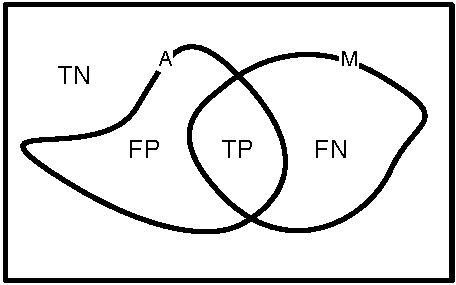
\includegraphics[height=.3\textwidth]{aor}~
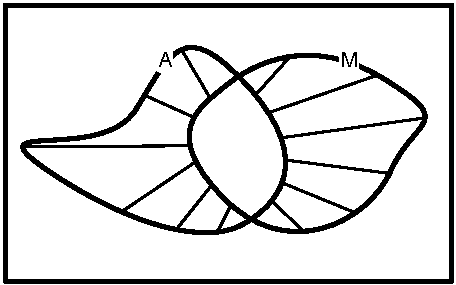
\includegraphics[height=.3\textwidth]{disterror}
\caption[Methodology evaluation.]{ Methodology evaluation. (a) Statistical hypothesis test errors confusion matrix. (b) 
Graphic representation of the statistical hypothesis test errors for assessing the performance in terms of area. (c) Graphical representation of the boundary distance performance measures.}
\label{fig:gtEval}
\end{figure}

\paragraph{Area based segmentation assessment metrics}
%When analyzing the areas described by the assessing segmentation $A$ and the reference segmentation $M$ (see fig.~\ref{fig:gtEval}b), 4 regions become apparent: \acf{tp},  \acf{tn},  \acf{fp},  and \acf{fn}; corresponding to the regions of the confusion matrix in figure~\ref{fig:gtEval}a.

When analyzing the areas described by the segmented region  to be assessed, $A$ and the manually delineated reference region $M$ (see fig.~\ref{fig:gtEval}b), 4 areas become evident: \acf{tp},  \acf{tn},  \acf{fp},  and \acf{fn}; corresponding to the regions of the confusion matrix in figure~\ref{fig:gtEval}a.


%\begin{table}[htdp]
%\caption{Statistical hypothesis test errors confusion matrix}
%\begin{center}
%\begin{tabular}{r||c|c|}
%&Positivie & Negative \\ \hline \hline
%Poisitve & \acf{tp} & \acf{fp}\\ \hline
%Negative & \acf{fn} & \acf{tn}\\
%\hline \hline
%\end{tabular}
%\end{center}
%\label{fig:TPTNconfusionMatrix}
%\end{table}%



%%
%%\begin{description}
%%\item[\acf{tp}]
%\paragraph{\acf{tp}}
%is found as the area in common ($A \wedge M$) between the two delineations $A$, $M$. 
%The \ac{tp} area corresponds to the correctly segmented areas belonging to the lesion.
%
%%\item[\acf{tn}] 
%\paragraph{\acf{tn}}
%is found as the area ($\overline{A} \wedge \overline{M}$) not belonging to either of the delineations $A$ nor $M$ . The \ac{tn} area corresponds to the correctly segmented areas belonging to the background of the image. 
%
%%\item[\acf{fp}] 
%\paragraph{\acf{fp}}
%is found as the area ($A \wedge \overline{M}$) belonging to the assessing segmentation $A$ and not as a part of the reference delineation $M$. \ac{fp} corresponds to the area wrongly labeled as a lesion since this area does not belong to the reference delineation.
%
%%\item[\acf{fn}] 
%\paragraph{\acf{fn}}
%is found as the area ($\overline{A} \wedge M$) corresponding to the reference delineation $M$ but not as a part of the assessing segmentation $A$. \ac{fn}
%corresponds to the areas of the true segmentation that have been missed by the segmentation under assessment.

%\end{description}
\vspace{15pt}
Area metrics (or indexes) for assessing the segmentation are defined as a dimensionless quotient relating the 4 regions (\ac{tp}, \ac{fp}, \ac{fn} and \ac{tn}) described by the segmentation outcome being assessed (denoted $A$ in fig:\ref{fig:gtEval}a) and the reference \ac{gt} segmentation (denoted $M$). Most of the indexes are defined within the interval $[0,1]$ and some works report their results as a percentage.

\begin{description}

\item[\acf{aov},] also known as overlap ratio, the \ac{jsc}~\cite{Gao:2012p14336} or \ac{si}~\cite{Shan:2012p14347}\footnote{Notice that \acf{si} is also used formulated as the \acf{dsc} in~\cite{Huang:2007p6100,Huang:2005p11636} which differs from the \ac{si} definition in~\cite{Shan:2012p14347}.}, is a common similarity index representing the percentage or amount of area common to the assessed delineation $A$ and the reference delineation $M$ according to equation~\ref{eq:aov}. 
The \ac{aov} metric has been used to assess the following works: \cite{Horsch:2001p6028,Gomez:2010p14339,AlemanFlores:2007p14310,Cui:2009p14325,massich2010lesion,Shan:2012p14347,hao2012combining,Liu:2010p14328}

\begin{equation}\label{eq:aov}
AOV = \frac{TP}{TP+FP+FN}=\frac{|A| \wedge |M|}{|A| \vee |M|} \qquad \in [0,1]
\end{equation}

\item[\acf{dsc},]
also found under the name of \ac{si}~\cite{Huang:2007p6100,Huang:2005p11636}\footnote{Notice that \acf{si} is also used formulated as the \acf{aov} in~\cite{Shan:2012p14347} which differs from the \ac{si} definition in~\cite{Huang:2007p6100,Huang:2005p11636}.},
is another widely used overlap metric similar to \ac{aov}. The difference between \ac{dsc} and \ac{aov} is that \ac{dsc} takes into account the \ac{tp} area twice, one for each delineation. 
The \ac{dsc} index is given by equation~\ref{eq:dsc} and the relation between \ac{aov} or \ac{jsc} and the \ac{dsc} similarity indexes is expressed by equation~\ref{eq:dsc2jsc}. Notice that the \ac{dsc} similiarity index is expected to be greater than the \ac{aov} index~\cite{gerard2013}. The \ac{dsc} metric has been used to assess the following works:\cite{gerard2013,Huang:2007p6100,Zhang:2010p14317,Huang:2005p11636}

\begin{equation}\label{eq:dsc}
DSC=\frac{2 \cdot TP}{2 \cdot TP + FP + FN}=\frac{2 | A \wedge M |}{|A| + |M|} \qquad \in [0,1]
\end{equation}

\begin{equation}\label{eq:dsc2jsc}
DSC=\frac{2 \cdot AOV}{1+AOV}
\end{equation}

\item[\acf{tpr},]
also known as the recall rate, sensitivity (at pixel level)~\cite{gerard2013,Jiang:2012p14354} or \ac{of}~\cite{Huang:2007p6100}, quantifies the amount of properly labeled pixels as lesion with respect to the amount of lesion pixels from the reference delineation (eq:~\ref{eq:tpr}). Notice that like the \ac{dsc}, this value always remains greater than \ac{aov} (or equal when the delineations are identical). The \ac{tpr} metric has been used to assess the following works:~\cite{Madabhushi:2003p6036,Huang:2007p6100,Shan:2012p14347,Jiang:2012p14354,Huang:2005p11636,Huang:2012p14313,Liu:2010p14328,Yeh:2009p11985}


\begin{equation}\label{eq:tpr}
TPR = \frac{TP}{TP+FN}= \frac{TP}{|M|} = \frac{|A| \wedge |M|}{|M|} \qquad \in [0,1]
\end{equation}

\item[\acf{ppv}]
corresponds to the probability that the pixel is properly labeled when restricted to those with positive test. It differentiates from \ac{tpr} since here the \ac{tp} area is regularized by the assessing delineation and not the reference, as can be seen in equation~\ref{eq:ppv}. \ac{ppv} is also greater than \ac{aov}. The \ac{ppv} metric is also used to assess the work in~\cite{gerard2013}.

\begin{equation}\label{eq:ppv}
PPV= \frac{TP}{FP+TP} = \frac{TP}{|A|}=\frac{|A| \wedge |M|}{|A|} \qquad \in [0,1]
\end{equation}


\item[\acf{nrv},]
also found as the Precission Ratio(PR)~\cite{Huang:2004p2092}, corresponds to the area of disagreement between the two delineations regularized by the size of the reference delineation, as described in equation:~\ref{eq:nrv}. Notice that the \ac{nrv} coefficient differs from $1-\ac{aov}$ since it is regularized by the reference delineation and not the size of the union of both delineations.
The \ac{nrv} metric has been used to assess the following works:~\cite{Gomez:2010p14339,Liu:2005p14341,Huang:2004p2092}.


\begin{equation}\label{eq:nrv}
NRV = \frac{|A \oplus M|}{|M|} \qquad \in \left[0, 1+\frac{A}{|M|}\right]
\end{equation}


\item[\acf{fpr},]
as reported in the presented work, is the amount of pixels wrongly labeled as lesion with respect to the area of the lesion reference, as expressed in equation~\ref{eq:fpr}. The \ac{fpr} metric has been used to assess the following works:\cite{Madabhushi:2003p6036,Shan:2012p14347,Huang:2012p14313,Liu:2010p14328,Yeh:2009p11985} The \ac{fpr} has also been found in its complementary form $1-TPR$ under the name of Match Rate (MR)~\cite{Huang:2004p2092}.

\begin{equation}\label{eq:fpr}
FPR'= \frac{FP}{TP + FN} = \frac{FP}{|M|}=\frac{|A \vee M - M|}{|M|} \qquad \in \left[0,\frac{A}{|M|}\right]
\end{equation}

Notice that the \ac{fpr} calculated in equation~\ref{eq:fpr} differs from the classic \ac{fpr2} obtained from the table in figure~\ref{fig:gtEval}a, which corresponds to the ratio between \ac{fp} and its column marginal ($FP+TN$), as indicated in equation~\ref{eq:fpr2}. The \ac{fpr2}, when calculated according to equation~\ref{eq:fpr2}, corresponds to the complement of specificity (described below).

\begin{equation}\label{eq:fpr2}
FPR= \frac{FP}{FP + TN} = 1-SPC \qquad \in [0,1]
\end{equation}

\item[\acf{fnr}]
corresponds to the amount of pixels belonging to the reference delineation that are wrongly labeled as background, as expressed in equation~\ref{eq:fnr}. Notice that it also corresponds to the inverse of the \ac{tpr} since $TP \cup FN = M$.
The \ac{fnr} metric has been used to assess the following works:
\cite{Madabhushi:2003p6036,Huang:2012p14313,Yeh:2009p11985}

\begin{equation}\label{eq:fnr}
FNR = \frac{FN}{|M|}=\frac{|A \vee M - A|}{|M|}=1-TPR \qquad \in [0,1]
\end{equation}

\item[Specificity] corresponds to the amount of background correctly labeled. Specificity is described in equation~\ref{eq:specificity} and is usually given as complementary information on the sensitivity (\ac{tpr}). Specificity corresponds to the complementary of the \ac{fpr2} when calculated according to equation~\ref{eq:fpr2}. The specificity index is also used to assess the work in~\cite{gerard2013,Jiang:2012p14354}.

\begin{equation}\label{eq:specificity}
SPC = \frac{TN}{TN+FP} = \frac{|\overline A \wedge \overline M|}{|\overline M|}=1-FPR \qquad \in [0,1]
\end{equation}
\end{description}

\paragraph{Boundary based segmentation assessment metrics}

Although the boundary assessment of the segmentations is less common than area assessment, it is present in the following works: \cite{AlemanFlores:2007p14310,Gomez:2010p14339,Gao:2012p14336,Madabhushi:2003p6036,
Shan:2012p14347,Zhang:2010p14317,Huang:2012p14313}. Like when assessing the segmentations in terms of area, the criteria for assessing disagreement between outlines are also heterogeneous which makes the comparison between works difficult. 
Unlike the area indexes, with the exception of the further introduced \ac{are} coefficient, which is also a dimensionless quotient, the rest of the boundary indexes or metrics are physical quantitative error measures and are assumed to be reported in pixels. Although some of the reported measures are normalized, they are not bounded by any means.

Zhang et al.~\cite{Zhang:2010p14317} propose using average contour-to-contour distance ($E_{cc}$) for assessing their work. However, no definition or reference is found on it. Huang et al.~\cite{Huang:2012p14313} propose using \ac{are}, defined in equation~\ref{eq:are}, where a set of $n$ radial rays are generated from the center of the reference delineation $C_0$ intersecting both delineations. The \ac{are} index consists of averaging the ratio between the distance of the two outlines $|C_s(i)-C_r(i)|$ and the distance between the reference outline and its center $|C_r(i)-C_0|$.

\begin{equation}\label{eq:are}
ARE = \frac{1}{n}\sum_{i=1}^{n} \frac{|C_s(i)-C_r(i)|}{|C_r(i)-C_0|}
\end{equation}

The rest of the works base their similitude indexes on the analysis of the \ac{md} coefficients. The \ac{md} is defined in equation~\ref{eq:md} and corresponds to the minimum distance between a particular point $a_i$ within the contour $A$ (so that $a_i \in A$) and any other point within the delineation $M$. 

\begin{equation}
\text{MD}(a_i,M) =\min_{m_j \in M}\Arrowvert a_i - m_j \Arrowvert 
\label{eq:md}
\end{equation}

\paragraph{\acf{hd},} or Hausdorff error, measures the worst possible discrepancy between the two delineations $A$ and $M$ as defined in \ref{eq:Hd}. Notice that it is calculated as the maximum of the worst discrepancy between $(A,M)$ and  $(M,A)$ since \ac{md} is not a symmetric measure, as can be observed in figure~\ref{fig:md}. The \ac{hd} as defined in equation~\ref{eq:Hd} has been used for assessing the segmentation results in Gao et al.~\cite{Gao:2012p14336}. Meanwhile, Madabhushi and Metaxas~\cite{Madabhushi:2003p6036} and Shan et al.~\cite{Shan:2012p14347} only take into account the discrepancy between the assessed delineation $A$ with reference delineation $M$, here denoted as \ac{hd}' (see eq.\,\ref{eq:Hd2}). In \cite{Madabhushi:2003p6036,Shan:2012p14347}, the \ac{hd}' is also reported in a normalized form $\frac{\text{HD}'}{\eta}$, where $\eta$ is the length of the contour of reference $M$.

\begin{equation}
\text{HD} (A,M) = \max \bigg \{ \max_{a_i \in A} \text{MD}(a_i,M), \max_{m_i \in M} \text{MD}(m_i,A)  \bigg \}
\label{eq:Hd}
\end{equation}
\begin{equation}
\label{eq:Hd2}
\text{HD'} (A,M) = \max_{a_i \in A} \text{MD}(a_i,M)
\end{equation}

\begin{figure}
\centering
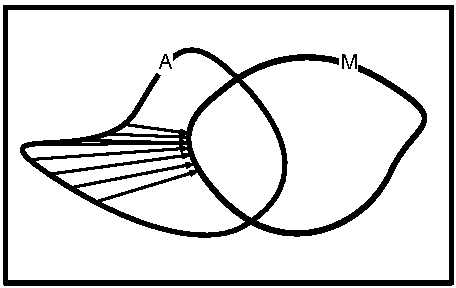
\includegraphics[height=.3\textwidth]{mdA-M}~
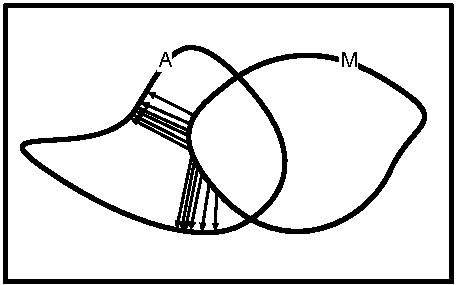
\includegraphics[height=.3\textwidth]{mdM-A}

\caption[Non-symmetry propoerty of the \ac{md} metric.]{Illustration of the non-symmetry property of the \acf{md} metric. (a) $\text{MD}(a_i,M)$, (b) $\text{MD}(m_i,A)$}
\label{fig:md}
\end{figure}

\paragraph{\acf{amed},} defined in equation~\ref{eq:amed}, is the average \ac{md} between the two outlines.~\cite{Gao:2012p14336}. Similar to the case of the \ac{hd}' distance, Madabhushi and Metaxas~\cite{Madabhushi:2003p6036} and Shan et al.~\cite{Shan:2012p14347} only take into account the discrepancy between the assessed delineation $A$ with reference to the delineation $M$ to calculate the \ac{amed}' index (see eq.\,\ref{eq:amed2}). The \ac{amed} index can be found under the name of Mean Error (ME) in~\cite{Madabhushi:2003p6036} and Mean absolute Distance (MD) in.~\cite{Shan:2012p14347}.

\begin{equation}
\text{AMED} (A,M) = \frac{1}{2}  \cdot  \Bigg [ 
 \frac{ \sum_{a_i \in A} \text{MD}(a_i,M)}{|A|} + \frac{ \sum_{m_i \in M} \text{MD}(m_i,A) }{|M|} \Bigg ]
\label{eq:amed}
\end{equation}
\begin{equation}
\label{eq:amed2}
\text{AMED'} (A,M)= \frac{ \sum_{a_i \in A} \text{MD}(a_i,M)}{|A|}
\end{equation}

\paragraph{\ac{pd},} used in~\cite{AlemanFlores:2007p14310,Gomez:2010p14339}, takes into account the \ac{amed} regularized with the area of the reference delineation according to equation~\ref{eq:pd}

\begin{equation}
\text{PD} (A,M) = \frac{1}{2 \sqrt{\frac{Area(M)}{\pi}}} \cdot  \Bigg [ 
 \frac{ \sum_{a_i \in A} \text{MD}(a_i,M)}{|A|} + \frac{ \sum_{m_i \in M} \text{MD}(m_i,A) }{|M|} \Bigg ] * 100
\label{eq:pd}
\end{equation}

\subsection[Multiple grader delineations ]{Multiple grader delineations ( Study of inter- and intra-observer segmentation variability)}\label{sec:multipleGT}
%\footnote{\color{red} I swear God that i had a paper using a metric that takes into account two (and only two) graders GT. But i don't find it !!!}

Assessing the true performance of a medical imaging segmentation procedure is, at least, difficult. Although method comparison can be achieved by assessing the methodologies with a common dataset and metric, true conclusions about the performance of the segmentation are questionable. Assessing segmentations of medical images is challenging because of the difficulty of obtaining or estimating a known true segmentation for clinical data. Although physical and digital phantoms can be constructed so that reliable \ac{gt} are known, such phantoms do not fully reflect clinical imaging data. An attractive alternative is to compare the segmentations to a collection of segmentations generated by expert raters. 

Pons et al.~\cite{gerard2013} analyzed the inter- and intra-observer variability of manual segmentations of breast lesions in \ac{us} images. In the experiment, a subset of 50 images is segmented by an expert radiologist and 5 expert biomedical engineers with deep knowledge of a breast lesion appearance in \ac{us} data. The experiment reported an \ac{aov} rate between $0.8$ and $0.852$ for the 6 actors. This demonstrates the large variability between \ac{gt} delineations; a fact that needs to be taken into account in order to draw proper conclusions about the performance of a segmentation methodology. However, having multiple \ac{gt} delineations to better assess the segmentations performance is not always possible. When possible, several strategies have been used to incorporate such information.

Cui et al.~\cite{Cui:2009p14325} tested the segmentation outcome against 488 images with two delineations provided by two different radiologists. The dataset is treated as two different datasets and the performance on both is reported.
Yeh et al.~\cite{Yeh:2009p11985} used a reduced dataset of 6 images with 10 different delineations accompanying each image. The performance for each image was studied in terms of reward average and variation of the 10 reference delineations.
Aleman-Flores et al.~\cite{AlemanFlores:2007p14310}, where a dataset of 32 image dataset with 4 \ac{gt} delineations provided by 2 radiologists (2 each) was available, assessed the segmentation method as if there were 128 ($32 \times 4$) images.

A more elaborate idea to estimate the underlying true \ac{gt} is proposed by Massich et al.~\cite{massich2010lesion} and Pons et al.~\cite{gerard2013}. Both works propose the use of \ac{staple} in order to determine the underlying \ac{gt} from the multiple expert delineations. \ac{staple} states that the ground truth and performance levels of the experts can be estimated by formulating the scenario as a missing-data problem, which can be subsequently solved using an \ac{em} algorithm. The \ac{em} algorithm, after convergence, provides the \acf{hgt} estimation that has been inferred from the segmentations provided by the experts as a probability map. Massich et al.~\cite{massich2010lesion} propose to assess the segmentation against a thresholded \ac{hgt} and weight the \ac{aov} index with the \ac{hgt}. The authors in~\cite{massich2010lesion} argued that apart from comparing the segmentation resulting from binarizing the greaders segmentation agreement, the amount of agreement the needs to be taken into account. This way, properly classifying a pixel with large variability within the graders produces less reward and miss classifying a pixel with great consensus penalizes.

